%Christopher Greene 
%Bonus question
%05/15/2025

\documentclass[12pt]{amsart}

%decrease margins 
\usepackage[top=.5in, left=1in, right=1in, bottom=1in]{geometry}
\usepackage{amsmath,amssymb,amsthm}
\usepackage{graphicx}
\usepackage{float}

%command for symbolic line integral 
\newcommand{\lineint}[1]{\int_C \vec{#1} \cdot d\vec{r}}

%command for symbolic surface integral 
\newcommand{\surfint}[1]{\iint_D {#1} \cdot d\vec{s}}

%command for vector notation
\newcommand{\vectr}[3]{\langle {#1} , {#2} , {#3} \rangle}

%command for div F 
\newcommand{\diver}[1]{\frac{\partial F_{#1}}{\partial {#1}}}

%get rid of the word abstract in the section
\renewcommand{\abstractname}{}



\title{Bonus problems}
\author{Christopher Greene}
\date{May 15, 2025}


\begin{document}

\maketitle

\begin{abstract}
    My primary resources were my notes from lectures , lab example problems and pauls notes. I combined these resources with AI so I could import these 
    resources into chatGPT and ask specific questions about the parts I did not understand, or where I made an error in a step when I got stuck.
\end{abstract}

\section{Problem 1}
%do not forget to add figures

Let $ \vec{F}(x,y,z) = \langle sin(x^2) , xz , z^2 \rangle $
Evaluate $\lineint{F}$ around the curve C of the intersection of the cylinder $ x^2 + y^2 = 4$ with 
the surface $z = x^2$ in the counter-clockwise direction as viewed from the top of the z-axis.

Use Stokes Theorem: \\
Which applies when: \\
-C is closed, simple and piecewise smooth \\
-Does not intersect \\
-Oriented counter clockwise when viewed from above. \\

Therefore for this problem we can say:
$\lineint{F} = \surfint{\mathrm{curl}\,\vec{F}}$ 
\[
\mathrm{Curl}(\vec{F}) = \begin{bmatrix}
    \vec{i} & \vec{j} & \vec{k} \\
    F_x     &  F_y    &  F_z    \\
    sin(x^2)&  xz     &  z^2    \\
\end{bmatrix}
\]

this yields:
$\surfint{\vectr{-x}{0}{z}}$

$d\vec{s}$ can be defined as $r_u \times r_v$ 

Our surface is given by the intersection between this cylinder and parabolic sheet.

\begin{figure}[H]
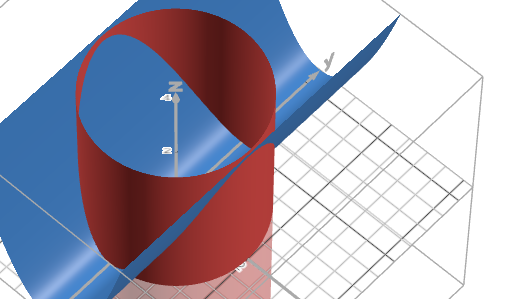
\includegraphics[width=0.5\textwidth]{Figure1.png}  
\caption{Intersection between cylinder and parabolic sheet}
\label{figure1}  
\end{figure}

We can parameterize this surface to get our surface s: 
Let x = u ,\, y = v and because $z = x^2$ \, $z = u^2$ \\
now we have $r(u,v) = \vectr{u}{v}{u^2}$ for u and v $\in x^2 + y^2 \leq 4$ \\ 
$r_u = \vectr{1}{0}{2u} \quad r_v = \vectr{0}{1}{0}$ \\
\[
r_u \times r_v = \begin{bmatrix}
    \vec{i}  &  \vec{j}   & \vec{k} \\
       1     &    0       &  2u     \\
       0     &    1       &  0      \\
\end{bmatrix}
\]

This gives our normal vector $\vec{n} = \vectr{-2u}{0}{1}$

to get the integrand: $\vectr{-u}{0}{u^2} \cdot \vectr{-2u}{0}{1}$

$\surfint{2u^2 + 2u} \\ 
 \surfint{3u^2}$ \\
let \quad $u = r\,cos\,(\theta) , v = r\,sin\,(\theta)$

we now have: \\ 
%dont use surface integral cmd do it manually 
$\int_{0}^{2\pi} \int_{0}^{0} 3r^2cos^2(\theta) \, dr \,d\theta$ \\
$\int_{0}^{2\pi} [\frac{3}{4}\,r^4cos^2(\theta)] \big|_0^2 \, d\theta$ \\
$\int_{0}^{2\pi} 12cos^2(\theta) \, d\theta$ \\
The double angle formula is given by: $cos^2(\theta) = \frac{1+cos(2\theta)}{2}$ \\
$12 \int_{0}^{2\pi} \frac{1+cos(2\theta)}{2}$ \\
$\int_{0}^{2\pi} 6+6cos(2\theta)$ \\
$6 \int_{0}^{2\pi} 1 + cos(2\theta)$ \\
$6[2\pi + \frac{1}{2}sin(2\theta)]$ \\
$12\pi + 3sin(4\pi)$ \\
Sin over any even number of pi over 1 period = 0 \\
$12\pi + 0 = 12\pi$ 




\section{Problem 2}
%do not forget to add figures

Let E be the solid region between the plane $z = 4$ and the parabolid $z = x^2 + y^2$
Let $\vec{F}(x,y,z) = \langle \frac{-1}{3}x^3 + e^{z^2} , \frac{-1}{3}y^3 +xsin(z) , 4z \rangle$
Let S be the surface that encloses E.
Find $\int \int_S \vec{F} \cdot d\vec{s}$

We can apply divergence theorem as E is an enclosed region between our paraboloid and our plane. Our parabolid is not closed but we can artificially close it through our limits of 
integration. 

Divergence theorem is given by $\surfint{\vec{F}} = \iiint_V \mathrm{div(\vec{F})} dV$

Our region is bounded by $z = 4 , z = x^2 + y^2$ as shown in figure 2. 

\begin{figure}[H]
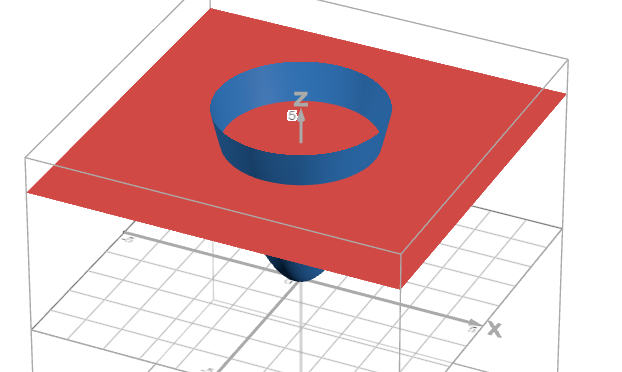
\includegraphics[width=0.5\textwidth]{Figure2.png}  
\caption{Intersection between paraboloid and plane}
\label{figure2}  
\end{figure}

%readability \newcommand{\diver}[1]{\frac{\partial F_[#1]}{\partial [#1]}}
$\mathrm{div}(\vec{F})= \diver{x} + \diver{y} + \diver{z}$

now that the problem is contextualized we break down the integral: \\
$\diver{x} = - x^2 \quad \diver{y} = -y^2 \quad \diver{z} = 4 \\
\iiint_V -x^2 - y^2 + 4 \, dV $ 
\\

The paraboloid itself that encloses the region has an open top but we can artificially enclose the paraboloid by limiting the upper bound to $z = x^2 + y^2$

let \\
$ x = rcos\theta \\ y = rsin\theta \\ z = x^2 + y^2 \\ z = r^2cos^2\theta + r^2sin^2\theta \\ z = r^2$ \\ 
because $z = x^2 + y^2 \quad r^2 = x^2 + y^2 \quad r = 2$ 

set up the bounds of integration: 
$ \int_{0}^{2\pi} \int_{0}^{2} \int_{4}^{r^2} \, -r^2cos^2\theta - r^2sin^2\theta + 4 r \, dz \, dr \, d\theta$

$ \int_{0}^{2\pi} \int_{0}^{2} \int_{4}^{r^2} \, -r^3cos^2\theta - r^3sin^2\theta + 4r \, dz \, dr \, d\theta$

$ \int_{0}^{2\pi} \int_{0}^{2} \, -zr^3cos^2\theta - zr^3sin^2\theta + 4zr \, \big|_4^{r^2} \, dr \, d\theta$

$ \int_{0}^{2\pi} \int_{0}^{2} \, -r^5cos^2\theta - r^5sin^2\theta + 4r^3 + 4r^3cos^2\theta + 4r^3sin^2\theta - 16r  \, dr \, d\theta$

$4r^3cos^2\theta + 4r^3sin^2\theta = 4r^3$

$ \int_{0}^{2\pi} \int_{0}^{2} \, -r^5cos^2\theta - r^5sin^2\theta + 8r^3 - 16r  \, dr \, d\theta$

%error in this line at integrating 8r^3 whiteboard looks wrong it is corrected here
$ \int_{0}^{2\pi} \, -\frac{1}{6}r^6cos^2\theta - \frac{1}{6}r^6sin^2\theta + 2r^4 - 8r^2  \, \big|_0^2 \, d\theta$

$ \int_{0}^{2\pi} \, -\frac{64}{6}cos^2\theta - \frac{64}{6}sin^2\theta  \, d\theta$

$ \frac{64}{6}\int_{0}^{2\pi} \, -cos^2\theta - sin^2\theta  \, d\theta$

Use trig substitutions: \\
$cos^2\theta = \frac{1+cos(2\theta)}{2}
sin^2\theta = \frac{1-cos(2\theta)}{2}$

$\frac{64}{6} \int_{0}^{2\pi} \frac{-1-cos(2\theta)}{2} - \frac{1-cos(2\theta)}{2} \, d\theta$ 

$\frac{64}{6} \int_{0}^{2\pi} -1 \, d\theta$ 

$\frac{64}{6} (-2\pi)$ 

$\frac{-128\pi}{6}$

$\frac{-64\pi}{3}$

Answer represents a volume so should be positive but is negative because I put r in the upper limit of integration instead of lower. 














\end{document}
